\documentclass[paper=a4, fontsize=11pt]{article}

%----------------------------------------------------------------------------------------
%	PACKAGES AND OTHER DOCUMENT CONFIGURATIONS
%----------------------------------------------------------------------------------------

\usepackage{amsmath,amsfonts,amsthm} % Math packages
\usepackage{sectsty} % Allows customizing section commands
\usepackage{authblk} % make multiple author
\usepackage{afterpage} % to make a blank page in document
\allsectionsfont{\normalfont\scshape} % Make all sections centered, the default font and small caps

\usepackage{fancyhdr} % Custom headers and footers
\pagestyle{fancyplain} % Makes all pages in the document conform to the custom headers and footers
\fancyhead{} % No page header - if you want one, create it in the same way as the footers below
\fancyfoot[L]{} % Empty left footer
\fancyfoot[C]{} % Empty center footer
\fancyfoot[R]{\thepage} % Page numbering for right footer
\renewcommand{\headrulewidth}{0pt} % Remove header underlines
\renewcommand{\footrulewidth}{0pt} % Remove footer underlines
\setlength{\headheight}{13.6pt} % Customize the height of the header

\numberwithin{equation}{section} % Number equations within sections (i.e. 1.1, 1.2, 2.1, 2.2 instead of 1, 2, 3, 4)
\numberwithin{figure}{section} % Number figures within sections (i.e. 1.1, 1.2, 2.1, 2.2 instead of 1, 2, 3, 4)
\numberwithin{table}{section} % Number tables within sections (i.e. 1.1, 1.2, 2.1, 2.2 instead of 1, 2, 3, 4)

\setlength{\parindent}{4em}
\setlength{\parskip}{1em}
\renewcommand{\baselinestretch}{1.5}

\usepackage{graphicx}
\graphicspath{ {images/} }

\usepackage{xepersian}
\setlatintextfont{Times New Roman}

%----------------------------------------------------------------------------------------
%	TITLE SECTION
%----------------------------------------------------------------------------------------

\newcommand{\horrule}[1]{\rule{\linewidth}{#1}} % Create horizontal rule command with 1 argument of height
\newcommand\blankpage{%
    \null
    \thispagestyle{empty}%
    \addtocounter{page}{-1}%
    \newpage}
\title{
\normalfont\normalsize

\includegraphics[scale=0.1]{aut}
\hspace{5cm}

\includegraphics[scale=0.1]{ceit} \\
\textsc دانشگاه صنعتی امیرکبیر \\
\textsc دانشکده مهندسی کامپیوتر و فناوری اطلاعات
\horrule{0.5pt} \\ [0.4cm] % Thin top horizontal rule
\huge سیستم تشخیص تقلب در بیمه \\ % The assignment title
\horrule{2pt} \\ [0.5cm] % Thick bottom horizontal rule
}

\author{{استاد راهنما :‌ دکتر رضا صفابخش} \\
{نگارنده : علیرضا حیدری}}

\date{\normalsize\today} % Today's date or a custom date

\pagenumbering{roman}

\begin{document}

\maketitle % Print the title
\thispagestyle{empty}
\clearpage
\afterpage{\blankpage}
\clearpage
\setcounter{page}{1}
\newpage


\section*{چکیده}
\par
در سبک زندگی امروزه، با توسعه انواع موانع و بلایای طبیعی و غیرطبیعی نیاز است تا راه‌حل هایی جهت بهبود مشکلات حاصل از این نوع 
بلایا ایجاد شود. صنعت بیمه جهت حل اینگونه بیمه ها ایجاد شد و باعث شد تا با ایجاد قراردادی بین یک بیمه‌گر و بیمه گذار بتوان راحت تر به حل این موارد پرداخت.
\par
صنعت بیمه با عقد قراردادی بین طرفین باعث می‌شود تا بیمه‌گر با پرداخت مبلغی از پرداخت مبلغ بیشتری در هنگام وقوع حادثه پیشگیری کند. این مبلغ را بیمه‌گر از مجموع پول‌های بدست آمده از قرارداد‌های کلی پرداخت می‌کند.
\par
باوجود این تلاش‌ها ممکن است در بسیاری از مواردی که بیمه‌ها ثبت می‌شوند در مراحل مختلف آن توسط افراد بیمه‌گر تخلفاتی صورت بگیرد که با تشخیص آن می‌توان به ادامه کار صنعت بیمه و افزایش اطمینان طرفین به یکدیگر کمک کرد.
\par
در این مقاله به مواردی که جهت ساخت سیستمی برای تشخیص تقلب در صنعت بیمه به آن‌ها نیازمندیم میپردازیم و سعی می‌کنیم این سیستم بهترین عملکرد ممکن را داشته باشد.


\newpage
\setcounter{page}{3}
\pagenumbering{arabic}
\tableofcontents
\newpage
\section{مقدمه}
\par
امـروزه فـروش بیمه اهمیت خـود را افـزایش داده اسـت و انـواع تـوسـعه هـا در این زمینه در حـال شکل گیري اسـت. بـا تـوسـعه این صـنعت و انـتقال مـوارد آن در بسـتروب و انـواع دیگر بسـترهـا، مشکلات فـراوانی در پی آن بـوجـود می‌آید. یکی از این مـوارد امکان تـقلب\footnote{fraud} در این سیستم اسـت بـه گـونـه اي که از مـتدوال تـرین نـوع این مـوارد، میتوان بـه گـرفـتن خـسارت از بیمه، آتـش سـوزي عـمدي، بـه صـورت مکرر اشـاره کرد
\par
فـروش و ثـبت عملیات هـاي بیمه‌اي بـه صـورت داده منجـر بـه دسـترسی داشـتن بـه اطـلاعـات عملیات هـاي بیمه‌اي یک کاربـر میشـود. میتـوان بـا بـررسی داده‌هـاي هـرکاربـر و نـحوه رفـتار او در رابـطه بـا خـرید بیمه و اسـتفاده از آن بـه نـحوه عملکرد پی بـرد و در صـورت وقـوع تـقلب، آن را تشخیص داد. تشخیص این تـقلب بـه الـگوریتم‌هـاي خـاص خـود و داده کاوي نیازمـند
است.
\par
در ادامه سعی می‌شود تا الگوریتم‌های لازم شناسایی و استفاده شوند و بتوان از آن ها در سیستم های تشخیص تقلب استفاده کرد.

\newpage

\section{صنعت بیمه}
\par
بیمه\footnote{Insurance} سازوکاری است که طی آن یک بیمه‌گر، بنا به ملاحظاتی تعهد می‌کند که زیان احتمالی یک بیمه‌گذار را در صورت وقوع یک حادثه در یک دوره زمانی خاص، جبران نماید یا خدمات مشخصی را به وی ارائه دهد؛ بنابراین، بیمه یکی از روشهای مقابله با ریسک است.
\par
طی یک قرارداد بیمه، ریسک مشخصی از یک طرف قرارداد (که بیمه‌گذار نامیده می‌شود) به طرف دیگر (که بیمه‌گر نامیده می‌شود) منتقل می‌گردد. بنا به تعریف، بیمه‌گر شخصی حقوقی است که در مقابل دریافت حق بیمه از بیمه‌گذار، جبران خسارت یا پرداخت مبلغ مشخصی را در صورت بروز حادثه تعهد می‌کند. در مقابل، بیمه‌گذار شخصی حقیقی یا حقوقی است که با پرداخت حق بیمه، جان، مال یا مسوولیت خود یا دیگری را تحت پوشش بیمه قرار می‌دهد.
\par
به موجب قانون بیمه ایران، بیمه عبارت است از قراردادی که به موجب آن یک طرف (بیمه گر) تعهد می‌کند در ازای پرداخت وجه یا وجوهی از طرف دیگر (بیمه گذار) در صورت وقوع یا بروز حادثه خسارت وارده بر او را جبران نموده یا وجه معینی را بپردازد. متعهد را بیمه گر، طرف تعهد را بیمه گذار و وجهی را که بیمه گذار به بیمه‌گر می‌پردازد حق بیمه و آنچه را که بیمه می‌شود موضوع بیمه نامند.

\subsection{انواع بیمه}
\par
در یک تقسیم‌بندی کلی بیمه به دو دسته بیمه های اجتماعی و بیمه‌های بازرگانی تقسیم‌بندی می‌شود.
مبحث تقلب به طور عمومی در بیمه‌های بازرگانی مطرح می‌شود که از انواع آن به موارد زیر می‌توان اشاره کرد:

\begin{itemize}
    \item بیمه آتش‌سوزی   
    \item بیمه حمل و نقل
    \item بیمه مسافرتی - بیمه سفر
    \item بیمه عمر
    \item بیمه حوادث
    \item بیمه بدنه اتومبیل
    \item بیمه شخص ثالث
    \item بیمه درمان
    \item بیمه سرطان
    \item بیمه کشتی
    \item بیمه هواپیما
    \item بیمه مهندسی
    \item بیمه پول
    \item بیمه مسوولیت
    \item بیمه اعتباری
\end{itemize}

\subsection{تقلب در صنعت بیمه}
\par
در سال ۲۰۰۲، موسسه تحقیقاتی فرانک به سفارش انجمن بیمه‌گران بریتانیا، تحقیقی با شرکت ۲۰۰۰ نفر انجام داد. هدف اصلی این تحقیق سنجش دیدگاه مردم در خصوص ادعاهای تقلبی در صنعت بیمه بود. هدف دیگری که از طراحی این تحقیق دنبال می‌شد، این بود که تقلب و سوءاستفاده از بیمه را جزو اقدامات خلاف قانون در جامعه مطرح کند. نتایج این تحقیق نشان می‌دهد که بخشی از تقلب و سوء استفاده در بیمه، ناشی از ناآگاهی و عدم شناخت مردم درباره چیزی است که درست است. بیشتر کسانی که در این تحقیق مورد پرسش قرار گرفته‌اند، درباره آنچه که رفتار درست تلقی می‌شود، اطلاع دقیقی نداشته‌اند. نتایج این تحقیق نشان داد که :
\begin{itemize}
    \item 
    اگرچه بیشتر پرونده‌ها و دعاوی بیمه ای درست و صحیح است، تقریبا نیمی از پرسش‌شوندگان احتمال تقلبی بودن یک ادعا را رد نکرده‌اند.
    \item
    احتمال وقوع تقلب بیمه‌ای بیشتر از سایر سوء استفاده‌هااست.
    \item
    در میان افراد شرکت کندده در تحقیق، در خصوص درست یا نادرست‌بودن اقداماتی مانند خریدن مال مسروقه یا رانندگی در حالت مستی، دیدگاه‌های متفاوتی وجود دارد.
\end{itemize}
\par
کلاهبرداری در بیمه اتومبیل از روش‌های مختلفی صورت می‌گیرد، برخی از شرکت‌ها اغراق در اعلام میزان خسارت و برخی دیگر سایر فعالیت‌های هدفمند، مانند تصادفات ساختگی، اسناد جعلی و ارائه اطلاعات نادرست را به‌عنوان مصادیق تقلب در‌نظر می‌گیرند.
بعضی از کلاهبرداری‌ها در صنعت بیمه کاملا آگاهانه و عمدی است. بیمه‌گذار ممکن است موجبات بروز خسارتی را فراهم آورد تا بدین طریق از محل بیمه‌نامه خود منفعتی کسب کند.
\par
به‌طور کلی، بیمه‌گذاران در دو موقعیت مرتکب تقلب می‌شوند: مورد اول، شرایطی است که در آن، فرد آگاهانه سعی در ایجاد خسارت یا اغراق در میزان و نوع خسارت دارد; به عنوان مثال، در یک سانحه تصادف ممکن است فرد بیمه‌گذار با توجه به حق‌بیمه‌ای که برای سالیان متمادی به شرکت بیمه پرداخت نموده است درصدد بهره‌برداری از فرصت برآید و با تجمیع کلیه زیان‌های پیشین با خسارت فعلی سعی در کسب موقعیت مالی بهتر کند. مورد دوم که ممکن است منجر‌به خسارت‌های جعلی گردد، مواردی است که بیمه‌گذار به صرف داشتن بیمه‌نامه احتیاط کمتری می‌کند. بدین معنی که گرچه ممکن است شخص قصد ایجاد خسارت یا اغراق در میزان آن را نداشته باشد، با این حال اقدام به انجام فعالیت‌هایی می‌کند که در صورت نداشتن بیمه‌نامه، این فعالیت‌ها را انجام نمی‌داد.

\newpage
\section{مراحل شناسایی تقلب}
یک مدل معمول و رایج برای تشخیص تقلب در نمودار ۱ قابل مشاهده است.
مراحل شامل شناسایی و غربال‌گری، تحقیق و بررسی، مذاکره با بیمه‌گذار یا طرح دعوی است که در روند ارزیابی خسارت ها اجرا می‌شود. روند ارزیابی خسارت‌ها با رخداد یک حادثه و اعلام گزارش به شرکت بیمه آغاز و با پرداخت یا عدم پرداخت خسارت پایان می‌یابد. عواملی چون عدم تمایل به ارائه اطلاعات صحیح از نشانه‌های کلاهبرداری است که در صورت اثبات تخلف منجر‌به عدم پرداخت خسارت می‌گردند.

\begin{figure}[h]
    \centering
    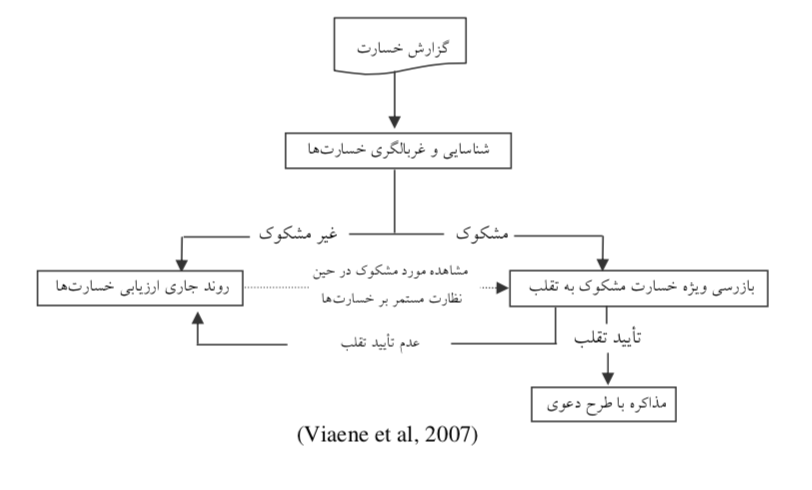
\includegraphics[scale=1]{model}
    \caption{مراحل تشخیص تقلب}
    \label{fig:model}
\end{figure}

\subsection{شناسایی و غربال‌گری\protect\footnote{identification and screening}}
\par
این مرحله جهت شناسایی و تفکیک خسارت‌های مشکوک به تقلب است. خسارت‌هایی که از این مرحله گذر‌ می‌کنند، طبق روال معمول و با حداقل هزینه‌های اداری ارزیابی می‌شوند، اما خسارت‌هایی که این امر مستلزم صرف زمان، هزینه و نیروی انسانی بیشتر است. بدون وجود سیستم های هوشمند، بررسی خسارت ها تنها براسا اطلاعات موجود درمورد بیمه‌گذار و خسارت وارده ممکن است. اما ازآنجا که معمولا جستجوی دستی در پرونده‌ها و موارد مشابه گذشته، بسیار مشکل و زمان‌بر است، کارشناسان خسارت باید براسا اطلاعات بسیار محدود و اغلب با اتکا به تجریبات به تصمیم‌گیری بپردازند.
معمولا داده‌ها از سه طریق قابل دستیابی اند:
\begin{itemize}
    \item
    گردآوری داده‌ها در مرحله صدور بیمه‌نامه از طریق فرم‌هایی که توسط بیمه‌گذاران پر می‌شوند، اطلاعاتی درمورد بیمه‌گذاران و اتومبیل بیمه شده از قبیل تاریخ تولد، نشانی، نوع اتومبیل، تاریخ اخذ گواهینامه رانندگی، نوع کاربری اتومبیل و ... که غالبا عوامل موثر در شناسایی ریسک تحت پوشش و تعیین نرخ مناسب در محاسبه حق‌ بیمه است را برای بیمه‌گر فراهم می‌آورد. همچنین این اطلاعات در آینده به همراه جزئیات خسارت در تکمیل پروفایل مشتریان استفاده می‌شود.
    \item
    گردآوری داده‌ها در مرحله ارزیابی خسارت‌ها که توسط کارشناسان مربوطه جهت پرداخت خسارت استفاده می‌شود، داده‌هایی از قبیل زمان، مکان، شرح وقوع و علت حادثه، شاهدان و مشخصات اتومبیل‌های ثالث(نوع، سال ساخت، سازنده) و ... را در اختیار شرکت بیمه قرار می‌دهند.
    \item
    گردآوری داده‌های موجود در پایگاه داده‌هایی که در صنعت اتومبیل اتومبیل اطلاعات مربوط به خودرو‌ها، مدل‌های آنها و هزینه خرید و تعمیر قطعات مختلف را در اختیار کارشناسان خسارت قرار می‌دهند. به کمک چنین پایگاه‌های داده‌ای، ارزیابان خسارت می‌توانند به سرعت مبالغ پرداخت را محاسبه کنند.
\end{itemize}

\subsection{تحقیق و بررسی\protect\footnote{investigation}}
تشخیص تقلبی‌بودن ادعا برعهده ارزیاب خسارت است که وی براساس تجربه، توانایی و خلاقیت خود این فرآیند را انجام می‌دهد. براساس تحقیقات تنیسن و سالساس\footnote{Tennyson \& Salsas, 2002}
 روش‌های رایج رسیدگی خسارت‌ها عبارت‌اند از: بازدید از محل، بررسی پیشینه، گزارش‌های واحدهای ویژه بازرسی و نظارت بر فعالیت‌های بیمه‌گذار

\subsection{مذاکره با بیمه‌گذار یا طرح دعوی}
اکثریت شرکت‌های بیمه ترجیح می‌دهند به همان روش‌های سنتی به بازرسی خسارت‌ها جهت تشخیص تقلب بپردازند، ولی با این‌حال در برخی از موارد نیاز به دادگاه خواهد بود. اما دعوی قضایی و بازرسی های ویژه معمولا مستلزم صرف هزینه و زمان زیادی است. معمولا شرکت‌های بیمه به‌دلیل تاثیری که ممکن است طرح دعوی در دادگاه و شکست احتمالی در آن، بر شهرت شرکت در بازار داشته باشد تمایلی به طرح دعوی در دادگاه‌ها ندارند.

\section{فراگیری ماشین و داده‌کاوی}
\par
با توجه به فراوانی اطلاعات در امروزه و در عصر حاضر مدیریت این داده های فراوان نیازمند دانش جدیدی است.
اطلاعات فراوانی در قالب پایگاه‌های داده ذخیره شده است که تبدیل آن‌ها به دانش مورد نیاز جهت تصمیم‌گیری، نیازمند ابزار‌های جدیدی است. روش‌های آماری برای تحلیل داده‌ها بیشتر برپایه استخراج شاخص‌های کمی استوار است. اگرچه این روش‌ها به صورت غیرمستقیم ما را به دانش مورد نیاز جهت تصمیم‌گیری سوق می‌دهند، اما درنهایت تفسیر نتایج آنها نیازمند تحلیل‌های انسانی است. روش‌های نوین تحلیل داده باید به دانش لازن و قابلیت تصمیم‌گیری براساس داده‌ها تجهیز شوند. جهت دستیابی به این هدف* محققین به ارائه ایده‌های جدیدی از فراگیری ماشین\footnote{Machine Learning} پرداخته اند.
با توجه به این ایده‌ها وظیفه فراگیری ماشین، تبدیل داده‌ها به دانش تصمیم‌گیری خواهد بود. همچنین براساس این ایده‌ها، ضرورت پیدایش یک حوزه تحقیقاتی جدید که داده‌کاوی\footnote{Data Mining} نام گرفته به وجود آمده است.
\par
داده کاوی فرآیند کشف الگو‌ها در داده‌ها است. این فرآیند باید خودکار یا نیمه‌خودکار باشد. الگو‌های شناسایی شده باید معتبر بوده و برای ما مزایایی از جمله مزایای اقتصادی داشته باشند. همچنین داده ها باید همواره در قالب کمیت های معتبر ارائه شوند.
استفاده از مدل های ریاضی برای شناسایی تقلب، این امکان را به متخصصین شرکت‌های بیمه می‌دهد که با صرف زمان و هزینه کمتری تشخیص دهند که ادعای خسارت اعلام شده از لحاظ آماری مشکوک به تقلب است یا خیر. در ادامه سه روش رگرسیون لجستیک، بیز ساده و درخت تصمیم‌گیری که از ابزار‌های رایج داده‌کاوی است معرفی و با استفاده از این روش‌ها مدل‌هایی برای شناسایی و دسته‌بندی خسارت‌های تقلبی بر روی داده‌های واقعی تعریف خواهد شد.

\newpage
\section{مطالعه تجربی}
\par
برای ساختن یک مدل ریاضی، نیاز به داده‌هایی از هر دو دسته ادعاهای جعلی و غیرجعلی داریم. در این بخش از این اطلاعات استفاده میکنیم و با سه الگوریتم ذکر شده به شناسایی موردهای دارای تقلب و مشکوک به آن می‌پردازیم.
\subsection{متغیر‌های مورد استفاده در مدل}
\par
در هریک از سه مدل مورد استفاده در شناسایی تقلب که در قبل بیان شد، جعلی یا غیرجعلی بودن یک پرونده، به عنوان متغیر وابسته درنظرگرفته می‌شود. مقدار ۱ برای متغیر وابسته به معنای جعلی‌بودن پرونده خسارت و مقدار ۰ به معنای غیرجعلی بودن آن پرونده است. در این مطالعه، فرآیند شناسایی تقلب با‌استفاده از شش متغیر مستقل صورت گرفته است. برای انتخاب متغیرها از روش ترکیبی استفاده شده است. روش ترکیبی از ترکیب دو روش پیش‌رونده و پس‌رونده تشکیل شده است. در این روش در هر مرحله از ورود متغیر‌ها به مدل، متغیر که کمترین ارتباط را با متغیر وابسته داشته باشد، حذف و متغیری که بیشتری ارتباط را داشته باشد، انتخاب می‌شود. همچنین برای بهتر‌شدن نتایج از نظرات کارشناسان بیمه اتومبیل نیز بهره گرفته شده است.
\par
اولین متغیر مستقل، سابقه بیمه‌ای هریک از بیمه‌گذاران در شرکت بیمه است. این متغیر به این دلیل انتخاب شده است که انتظار می‌رود احتمال ارتکاب تقلب توسط بیمه‌گذارانی که سابقه بیمه‌ای بیشتری در یک شرکت بیمه دارند، کمتر باشد.
بنابراین یک رابطه معکوس بین این متغیر و متغیر وابسته وجود دارد.
\par
دومین متغیر مستقل، تعداد ادعاهای خسارت بیمه‌گذاران در طول دوره سابقه بیمه است. تعداد ادعاهای خسارت بیشتر توسط یک بیمه‌گذار می‌تواند به این معنا باشد که بیمه‌گذار از بیمه‌نامه به‌منظور مقاصد سودجویانه استفاده کرده باشد. ازاین‌رو بین این متغیر و متغیر وابسته یک رابطه مستقیم وجود خواهد داشت.
\par
سومین متغیر مستقل، فاصله زمانی بین وقوع حادثه تا اعلام خسارت به شرکت بیمه از سوی بیمه‌گذار است. فرض شده است که هرچه این فاصله زمانی طولانی‌تر باشد، احتمال تقلب بیشتر افزایش خواهد یافت. بنابراین یک رابطه مستقیم بین این متغیر و متغیر وابسته وجود خواهد داشت.
\par
چهارمین متغیر مستقل، وضعیت کروکی خسارت رخ داده است. مقدار ۱ برای این متغیر به معنی نداشتن کروکی و مقدار ۰ به معنی داشتن کروکی است. این متغیر به این‌دلیل انتخاب شده است که با حضور پلیس در صحنه حادثه، شانس تقلب از قبیل صحنه‌سازی کاهش می‌یابد.

\subsection{روش رگرسیون لجستیک\protect\footnote{regression logistic}}
زمانی که متغیر وابسته، متغیری کیفی با دو سطح باشد، مدل‌های رگرسیون معمولی قابل استفاده نیستند. در این‌گونه موارد معمولا از رگرسیون لجستیک استفاده می‌شود. مدل رگرسیون لجستیک به‌این‌صورت تعریف می‌شود:
\begin{align}
\begin{split}
    logit(\frac{p}{1-p}) = \beta_{0} + \beta_{1}X_{1} + ... + \beta_{d}X_{d} 
\end{split}
\end{align}
که در این مدل  X‌ها متغیر های وابسته و p احتمال مشاهده مقدار ۱ برای متغیر وابسته به شرط مشاهده مقادیر متخلف x است.
\par
ضرایب رگرسیونی در این حالت با فرض دوجمله‌ای بودن توزیع متغیر وابسته از روش حداکثر درست‌نمایی برآورد می‌شوند. باتوجه به اینکه در این تحقیق متغیر وابسته(وضعیت پرونده خسارت) یک متغیر دو سطحی است، از رگرسیون لجستیک برای تشخیص جعلی یا غیرجعلی بودن پرونده‌های خسارت استفاده شده است. با استفاده از رگرسیون لجستیک پیش‌رو متغیر‌هایی که نقش مهم‌تری در تعیین وضعیت پرونده خسارت داشتهآند، شناسایی و وارد مدل شده‌اند. در گام اول مبلغ کل پرونده خسارت و مقدار ثابت در مدل قرار گرفته‌اند. در گام های دوم و سوم به ترتیب متغیر های فاصله زمانی وقوع حادثه تا اعلام خسارت و نوع خسارت به مدل افزوده شده‌اند.
\begin{figure}[h]
    \centering
    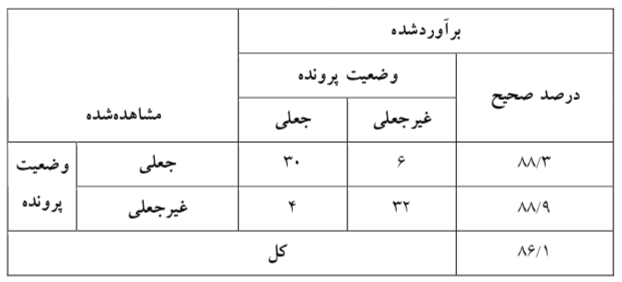
\includegraphics[scale=1]{table-r}
    \caption{دقت مدل در شناسایی وضعیت پرونده‌های خسارت با استفاده از رگرسیون لجستیک}
    \label{fig:table-r}
\end{figure}

\subsection{روش بیز ساده\protect\footnote{simple order}}
بیز ساده، شکل بسیار مقدماتی از مدل احتمال بیزی است. احتمال رخداد هریک از نتایج نهایی، براساس احتمالات رخداد متغیرهای مستقل به شرط رخداد همان نتیجه به‌دست‌می‌آید. فرض ما بر این است که احتمال رخداد هریک از متغیرهای مستقل به شرط رخداد یک نتیجه نهایی خاص، مستقل از احتمال رخداد سایر متغیرهای مستقل به شرط رخداد همان نتیجه باشد. عملکرد بیز ساده دسته کننده\footnote{Naive Bayes Classifier} بر فرضیات استفلال قوی استوار است. یعنی اینکه احتمال رخداد یک صفت روی احتمال سایر صفت‌ها بی‌تاثیر است. تئوری بیز امکان محاسبه احتمال پسین را برمبنای احتمالات پیشین فراهم می‌کند. در مدل احتمال بیر اگر h یک پیشامد و D مشاهدات باشد آنگاه خواهیم داشت:
\begin{align}
\begin{split}
    P(h|D) = \frac{P(D|h)P(h)}{P(D)}
\end{split}
\end{align}
که در آن P(h) احتمال رخداد h، P(D) احتمال رخداد D، P(D|h) احتمال رخداد D به شرط رخداد h و P(h|D) احتمال رخداد پیشامد h به شرط رخداد D است. در مواردی که مجموعه‌ای از پیشامدهای H وجود داشته باشد و بخواهیم محتمل ترین فرضیه را از میان آنان انتخاب کنیم، از فرضیه حداکثر احتمال\footnote{Maximum A Posteriori hypothesis (MAP)} استفاده می‌شود که رابطه آن به این شکل است:
\begin{align}
\begin{split}
    h_{MAP} = arg max P(h|D) \\
            = arg max \frac{P(D|h)P(h)}{P(D)}\\
            = arg max P(D|h)P(h)\\
\end{split}
\end{align}
\begin{figure}[h]
    \centering
    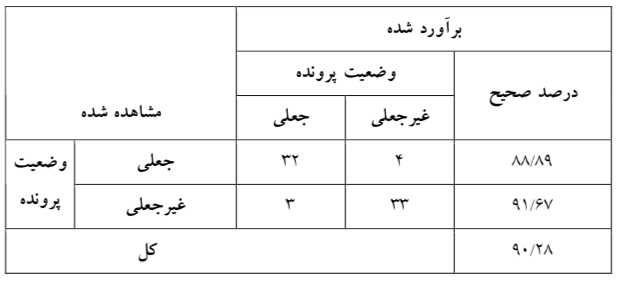
\includegraphics[scale=1]{table-b}
    \caption{دقت مدل در شناسایی وضعیت پرونده‌های خسارت با استفاده از مدل بیز ساده}
    \label{fig:table-b}
\end{figure}

\subsection{درخت تصمیم\protect\footnote{decision tree}}
\par
درخت تصمیم از ابزار‌‌های داده‌کاوی است که در رده‌بندی داده‌های کیفی استفاده می‌شود. در درخت تصمیم، درخت کلی به‌وسیله خردکردن داده‌ها به گره‌هایی ساخته می‌شود که مقادیری از متغیر‌ها را در خود جای می‌دهند. با ایجاد درخت تصمیم براساس داده‌های پیشین که رده آنها معلوم است، می‌توان داده‌های جدید را دسته بندی کرد. درخت تصمیم دارای قابلیت فهم بالا و سرعت مناسب در یادگیری الگو بوده و می‌توان از آن برای کشف تقلب در شرکت‌های بیمه استفاده کرد.
\par
هدف از استفاده از درخت تصمیم در این تحقیق، طبقه بندی داده‌های خسارت جدید در بیمه اتومبیل است. معیار‌های مختلفی برای تعیین صفتی که خردکردن داده‌ها باید براساس آن انجام شود، وجود دارد که از آن جمله می‌توان به معیار‌های بهره اطلاعاتی \footnote{ّInformation Gain}
، نسبت بهره\footnote{Gain Ratio}و شاخص جینی\footnote{Gini Index} اشاره کرد.
\begin{figure}[h]
    \centering
    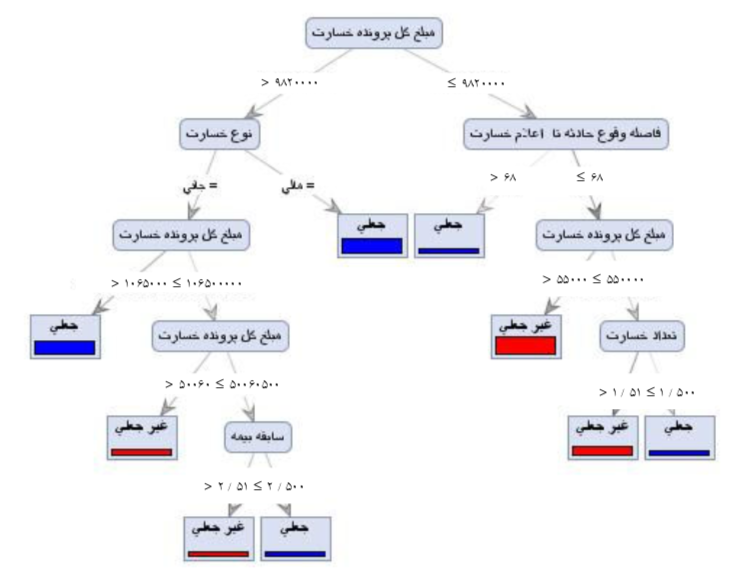
\includegraphics[scale=0.7]{dt}
    \caption{دقت مدل در شناسایی وضعیت پرونده‌های خسارت با استفاده از مدل بیز ساده}
    \label{fig:dt}
\end{figure}
\par
در ادامه با اعمال این مدل بر روی داده‌های اولی، نتایج زیر جهت بررسی دقت مدل به دست آمده است:
\begin{figure}[h]
    \centering
    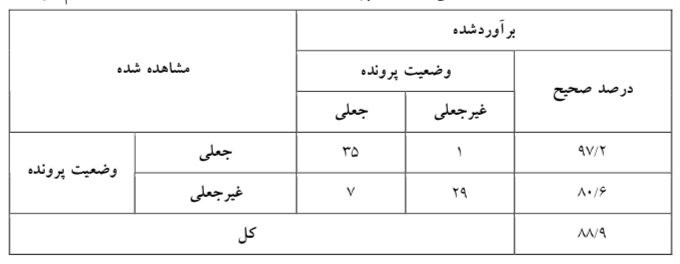
\includegraphics[scale=0.7]{table-dt}
    \caption{دقت مدل در شناسایی وضعیت پرونده‌های خسارت با استفاده از مدل بیز ساده}
    \label{fig:table-dt}
\end{figure}

\section{نتیجه گیری}
در این مقاله سه روش داده‌کاوی رگرسیون لجستیک، بیز ساده و درخت تصمیم برای ساخت مدل‌هایی جهت شناسایی ادعاهای خسارت تقلبی در بیمه اتومبیل معرفی شدند. در ادامه این روش‌ها بر روی داده‌های واقعی آزمایش و کارایی هر روش سنجیده شد. روش بیز ساده با دقت ۹۰.۲۸ درصد در شناسایی صحیح جعلی یا غیرجعلی بودن پرونده های خسارت بهترین کارایی را در مقایسه با دو روش درخت تصمیم با دقت کلی ۸۸.۹ درصد و رگرسیون لجستیک با دقت کلی ۸۶.۱ درصد داشت. البته باید به این نکته توجه داشت که در مدل بیز ساده برای تشخیص جعلی یا غیرجعلی بودن هر خسارت، شش متغیر و در مدل درخت تصمیم، پنج متغیر حضور دارند. این در حالی است که تصمیم گیری در مدل رگرسیون لجستیک برمبنای سه متغیری است که بیشترین همبستگی را با متغیر وابسته دارند.

\newpage
\section{پیوست‌ها}
\subsection{پیوست۱. جدول متغیر‌های مورد استفاده در مدل}

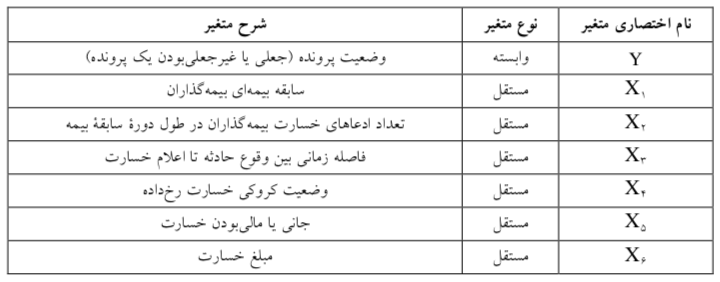
\includegraphics[scale=1]{p1}
\subsection{پیوست۲. ضرایب متغیرهای مدل و مقادیر P مقدار متناظر}
ضرایب هریک از متغیر‌های واردشده در مدل رگرسیون لجستیک و همچنین مقدار ثابت مدل همراه با مقادیر p مقدار آن ها در جدول نشان داده شده است.

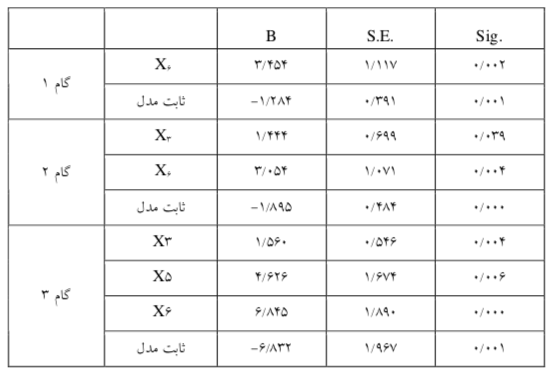
\includegraphics[scale=1]{p2}

\newpage
\section{منابع}
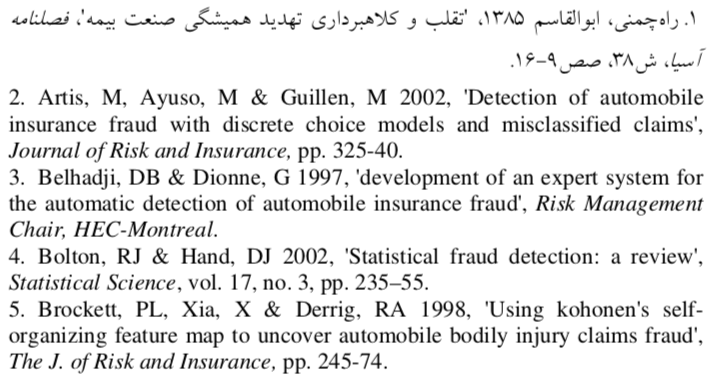
\includegraphics[scale=1]{resources}


\end{document}